\section{}

Wir geben den beiden Funktionen ein zusätzliches Argument \texttt{err}, mithilfe dessen entschieden wird, wann die Funktion abbricht; standardmäßig ist dieser Wert bei $10^{-6}$.

\lstinputlisting[style=pythoncode, firstline = 1, lastline = 19]{chapter_04/exercise_04_13.py}

Wir testen die beiden Funktionen an der gegebenen Funktion
\[
    f(x)
  = \sin(4x - 1) + x + x^{20} - 1.
\]
Hierfür plotten wir die Funktion zunächst mithilfe des folgenden Codes:

\lstinputlisting[style=pythoncode, firstline = 23, lastline = 31]{chapter_04/exercise_04_13.py}

Wir wählen das Intervall $[-1.1, 1.1]$, da die Funktion $f$ außerhalb dieses Intervalls zu groß wird.
Wir erhalten den folgenden Graphen:

\begin{center}
  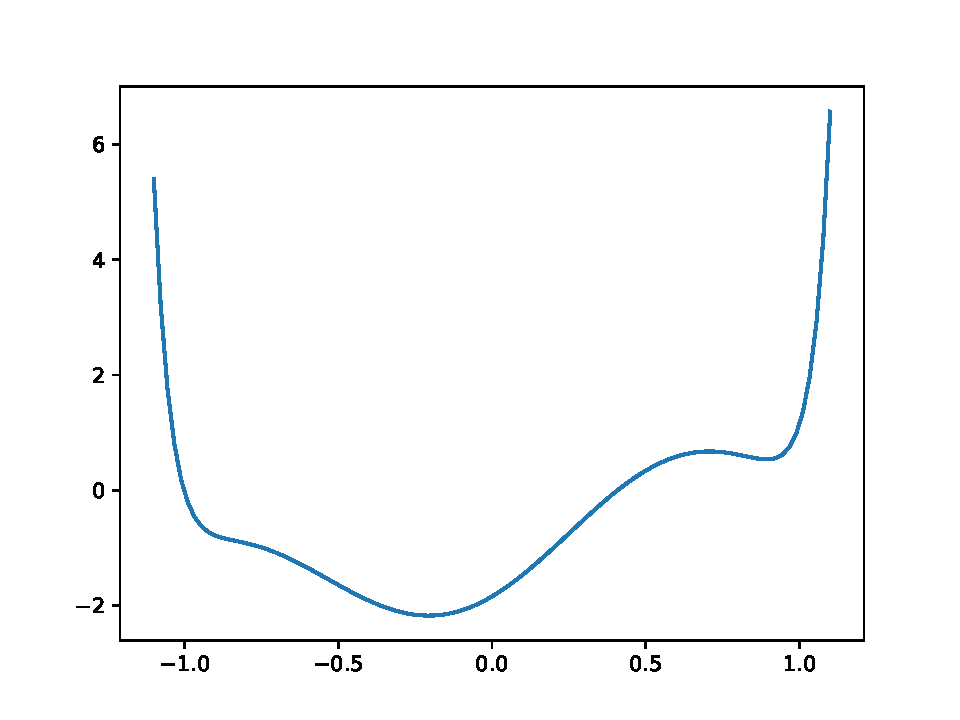
\includegraphics[width = 0.8\textwidth]{chapter_04/exercise_04_13_figure.pdf}
\end{center}

Anhand des Graphen sind zwei Nullstellen zu erkennen, jeweils in der Nähe von $-1$ und $0.4$.
Wir berechnen die Nullstellen nun mit dem folgenden Code:
  
\lstinputlisting[style=pythoncode, linerange={33-34, 38-39}]{chapter_04/exercise_04_13.py}

Wir erhalten den folgende Output:

\begin{consoleoutput}
  $ python exercise_04_13.py
  The roots with bisect_it are -1.002246916294098 and 0.4082937240600586.
  The roots with bisect_rec are -1.002246916294098 and 0.4082937240600586.
\end{consoleoutput}
